\thetitle{ Visualização de dados de honeypots }{ Visualização de dados de honeypots }
\thisyear{2015}
\author{Alexandre Or Cansian Baruque}
\principaladvisor{Prof. Dr. Paulo Licio de Geus}
\coadvisor{Prof. Dr. André Abed Grégio}


\beforepreface
\begin{oresumo}
O projeto tem como objetivo a implantação de um sistema para o tratamento e visualização de dados coletados por meio de sensores participantes de uma infra-estrutura de coleta de programas maliciosos.

Esse sistema foi desenvolvido fazendo o uso de tecnologias Web para o desenvolvimento de um serviço de visualização dos dados que correlaciona a posição geográfica da origem do potencial ataque com os registros desses ataques e suas respectivas datas e horas das coletas.

O uso funcionalidades integradas no sistema proposto pelo presente projeto permitirá que um analista consiga identificar os padrões e as tendências das atividades maliciosas registradas, tornando possível conclusões acerca dos dados observados.
\end{oresumo}
\afterpreface   


\chapter{Introdução}
Os programas maliciosos (\emph{malwares}) representam uma das maiores ameaças aos usuários e aos sistemas conectados à Internet. 

A facilidade da geração de novos exemplares a partir de um malware já existente, as chamadas variantes, dificulta a atuação dos mecanismos de defesa, tanto na criação de vacinas quanto no processamento das centenas de milhares de variantes em operação. Por exemplo, no caso de antivírus com detecção baseada em assinaturas é geralmente necessário a atuação de um analista humano que descubra um modo de detecção para um dado malware, e  então, produza a assinatura em questão. Para tanto, o analista também precisa ter em mãos a variante ainda não detectada.

A fim de obter programas maliciosos e as suas variantes, necessita-se de uma infraestrutura de coleta distribuída. A motivação principal para essa infraestrutura é a de obter e armazenar exemplares dos malwares em circulação no Brasil para análises posteriores melhorando as atuações dos mecanismos de defesa. 

Uma vez tendo acesso aos exemplares de malwares armazenados, pretende-se obter informações acerca dos tipos de malwares que atacam as redes brasileiras que possuem sensores de coleta (honeypots). 

As informações obtidas desses honeypots de coleta incluem tráfego de rede, registros de auditoria (logs) das vulnerabilidades exploradas e tipos de ataques utilizados no comprometimento dos serviços/sistemas e do binário que representa o programa malicioso. De posse de tais informações é possível representá-las  por meio de técnicas de visualização e disponibilizá-las por meio de uma arquitetura Web, permitindo a observação imediata de tendências ataques de uma maneira local (em cada rede) e global (conjunto das redes com sensores), além de geração de estatísticas.



\chapter{Atividades desenvolvidas}
Para alcançar os objetivos propostos no projeto, as seguintes atividades foram desenvolvidas:

\begin{enumerate}
\item Estudo de conceitos sobre visualização de dados através do uso de plataformas de desenvolvimento Web, como Django e Javascript. Em específico, foi estudado extensivamente o uso de bibliotecas para D3js\cite{d3js} (Data Driven Documents) e Jvectormap.\\
\item Definição da arquitetura a ser adotada para a implantação da infra-estrutura básica utilizada pelo servidor Web utilizado para a visualização dos dados e em outros sistemas necessários para a administração dos serviços.\\
\item Instalação das ferramentas e outros programas (e suas dependências) necessários para a implementação de um protótipo em uma máquina desktop provida pelo coorientador.\\
\end{enumerate}

Ao longo de todas as atividades desenvolvidas foi també́m feita a documentação do projeto, assim como outros relatórios e atividades requeridas (demonstração, levantamento de dados, etc).


\chapter{Metodologia}
No início do projeto foi necessário um estudo preliminar que permitiu obter conhecimentos para tomada de decisões acerca da arquitetura inicial, tais como escolha de ferramentas e plataformas de desenvolvimento a serem utilizadas.
Para tanto, observaram-se as ferramentas e os sistemas para visualização de dados de segurança já existentes, entre os quais as disponíveis pelos Projetos Honeynet\cite{honeynet}, Norse\cite{ipviking} e DioneaFR\cite{dioneaefr}, visto que os objetivos e as funcionalidades providas por essas ferramentas possuem componentes similares aos propostos no presente projeto. Entretanto, tais ferramentas/sistemas são limitados em certos aspectos, por exemplo: tipo e abrangência de dados, necessidade de compartilhamento de informações remotamente, entre outros, o que gera a necessidade de desenvolvimento de um sistema interno, de acesso controlado e extensível para os requisitos específicos dos dados coletados.
Após essa análise inicial e tendo definido as ferramentas a serem utilizadas, o enfoque do estudo foi em adquirir proficiência nas plataformas de desenvolvimento e ferramentas escolhidas para uso no projeto: Django, Jquery, Jvectormap, D3js, GeoIP, iNotify.

Para o controle de versão dos componentes de có́digo produzidos ao longo do projeto foi utilizado o sistema \emph{git}. Tais có́digos são armazenados em um repositó́rio privado criado no GitHub através de uma conta de estudante habilitada pelo bolsista. O repositó́rio consiste de dois ramos: o ramo mestre, no qual se mantém a versão mais atual do projeto com suas funcionalidades mais recentes, e o ramo demonstração, onde fica a ultima versão estável com o objetivo de ser utilizada para demonstrações funcionais do protótipo do sistema.

O framework Django\cite{django} em linguagem Python foi escolhido para constituir da infra-estrutura principal do projeto, tendo como função prover serviços de administração no back-end, assim como servir o có́digo em JavaScript a ser executado pelo cliente em um navegador Web. O Django também permite um fácil gerenciamento da base de dados (sqlite3) através da criação de procedimentos para administração. Foram desenvolvidas rotinas em shell script para consolidar os dados coletados na base de dados por meio dos procedimentos mencionados.

Uma arquitetura REST (Representational State Transfer) foi implantada fazendo uso de funcionalidades do Django, implicando que o acoplamento entre o cliente e o servidor não seja tão rígido, permitindo assim que modificações sejam feitas em ambos os lados sem muito impacto ao restante do sistema. O sistema implementado sobre tal arquitetura realiza consultas na base de dados e serializa os dados para serem encaminhados ao cliente executando có́digo JavaScript no formato JSON.

Para solucionar o problema de relacionar o endereço IP de origem do ataque com sua posição geográfica no mundo real, utilizou-se a ferramenta GeoIP\cite{geoip}, que permite baixar uma base relacional de IPs e latitude/longitude. Com isso, é possível traduzir a maioria dos endereços para localizações no mapa, obtendo também o país e a cidade de origem.

A visualização dos dados pelo cliente foi realizada pelo uso de bibliotecas de có́digo aberto baseados em JavaScript, sendo elas: jVectorMap\cite{jvectormap}, que permite a fácil criação e modificação de mapas interativos; D3js para a geração de gráficos contendo estatísticas gerais sobre os dados coletados; jQuery\cite{jquery}, que permite a criação de elementos de interface para prover interação com o usuário.

Um protótipo do sistema foi instalado em uma máquina provida pelo coorientador, a qual já continha dados de segurança coletados em um projeto envolvendo outro bolsista (infraestrutura distribuída para coleta e análise de dados de honeypots). Nesta máquina, os procedimentos previamente instalados fazem o polling dos dados coletados por sensores distribuídos e os agrega em uma estrutura no sistema de arquivos. Com todos os sistemas em funcionamento, o serviço Web que consome e processa tais dados atualiza sua informações de forma autônoma, provendo a visualização desejada.

\chapter{Resultados}
O resultado final foi um protótipo de um sistema cuja ferramenta principal permite a visualização de dados de potenciais ataques a protocolos de rede e aplicações de sistema, bem como de servidores comprometidos realizando o provimento de có́digos maliciosos para sensores distribuídos. A visualização desses dados é feita em um mapa, no qual são correlacionadas a origem do ataque (coordenadas geográficas do endereço IP obtido) com a frequência das ocorrências do ataque em questão (raio do círculo impresso em sua coordenada específica).

O mapa permite observar os dados sobre os ataques em uma dimensão temporal, atualizando as informações de acordo com o horário no qual tais dados foram coletados pelos sensores. Dessa forma, pode-se observar as tendências dos tipos de ataques no decorrer do dia, analisando-se os protocolos, serviços e locais de origem.
Desenvolveu-se uma imagem em máquina virtual para VirtualBox. A configuração desta máquina virtual já está corretamente aplicada com todos os requisitos para o funcionamento adequado do servidor Web utilizado no provimento da visualização de dados formatados de acordo com os requisitos do projeto. O desenvolvimento da máquina virtual citada tem como objetivo armazenar a ferramenta de uma forma portátil para ser utilizada em demonstrações. 

\begin{figure}
\center
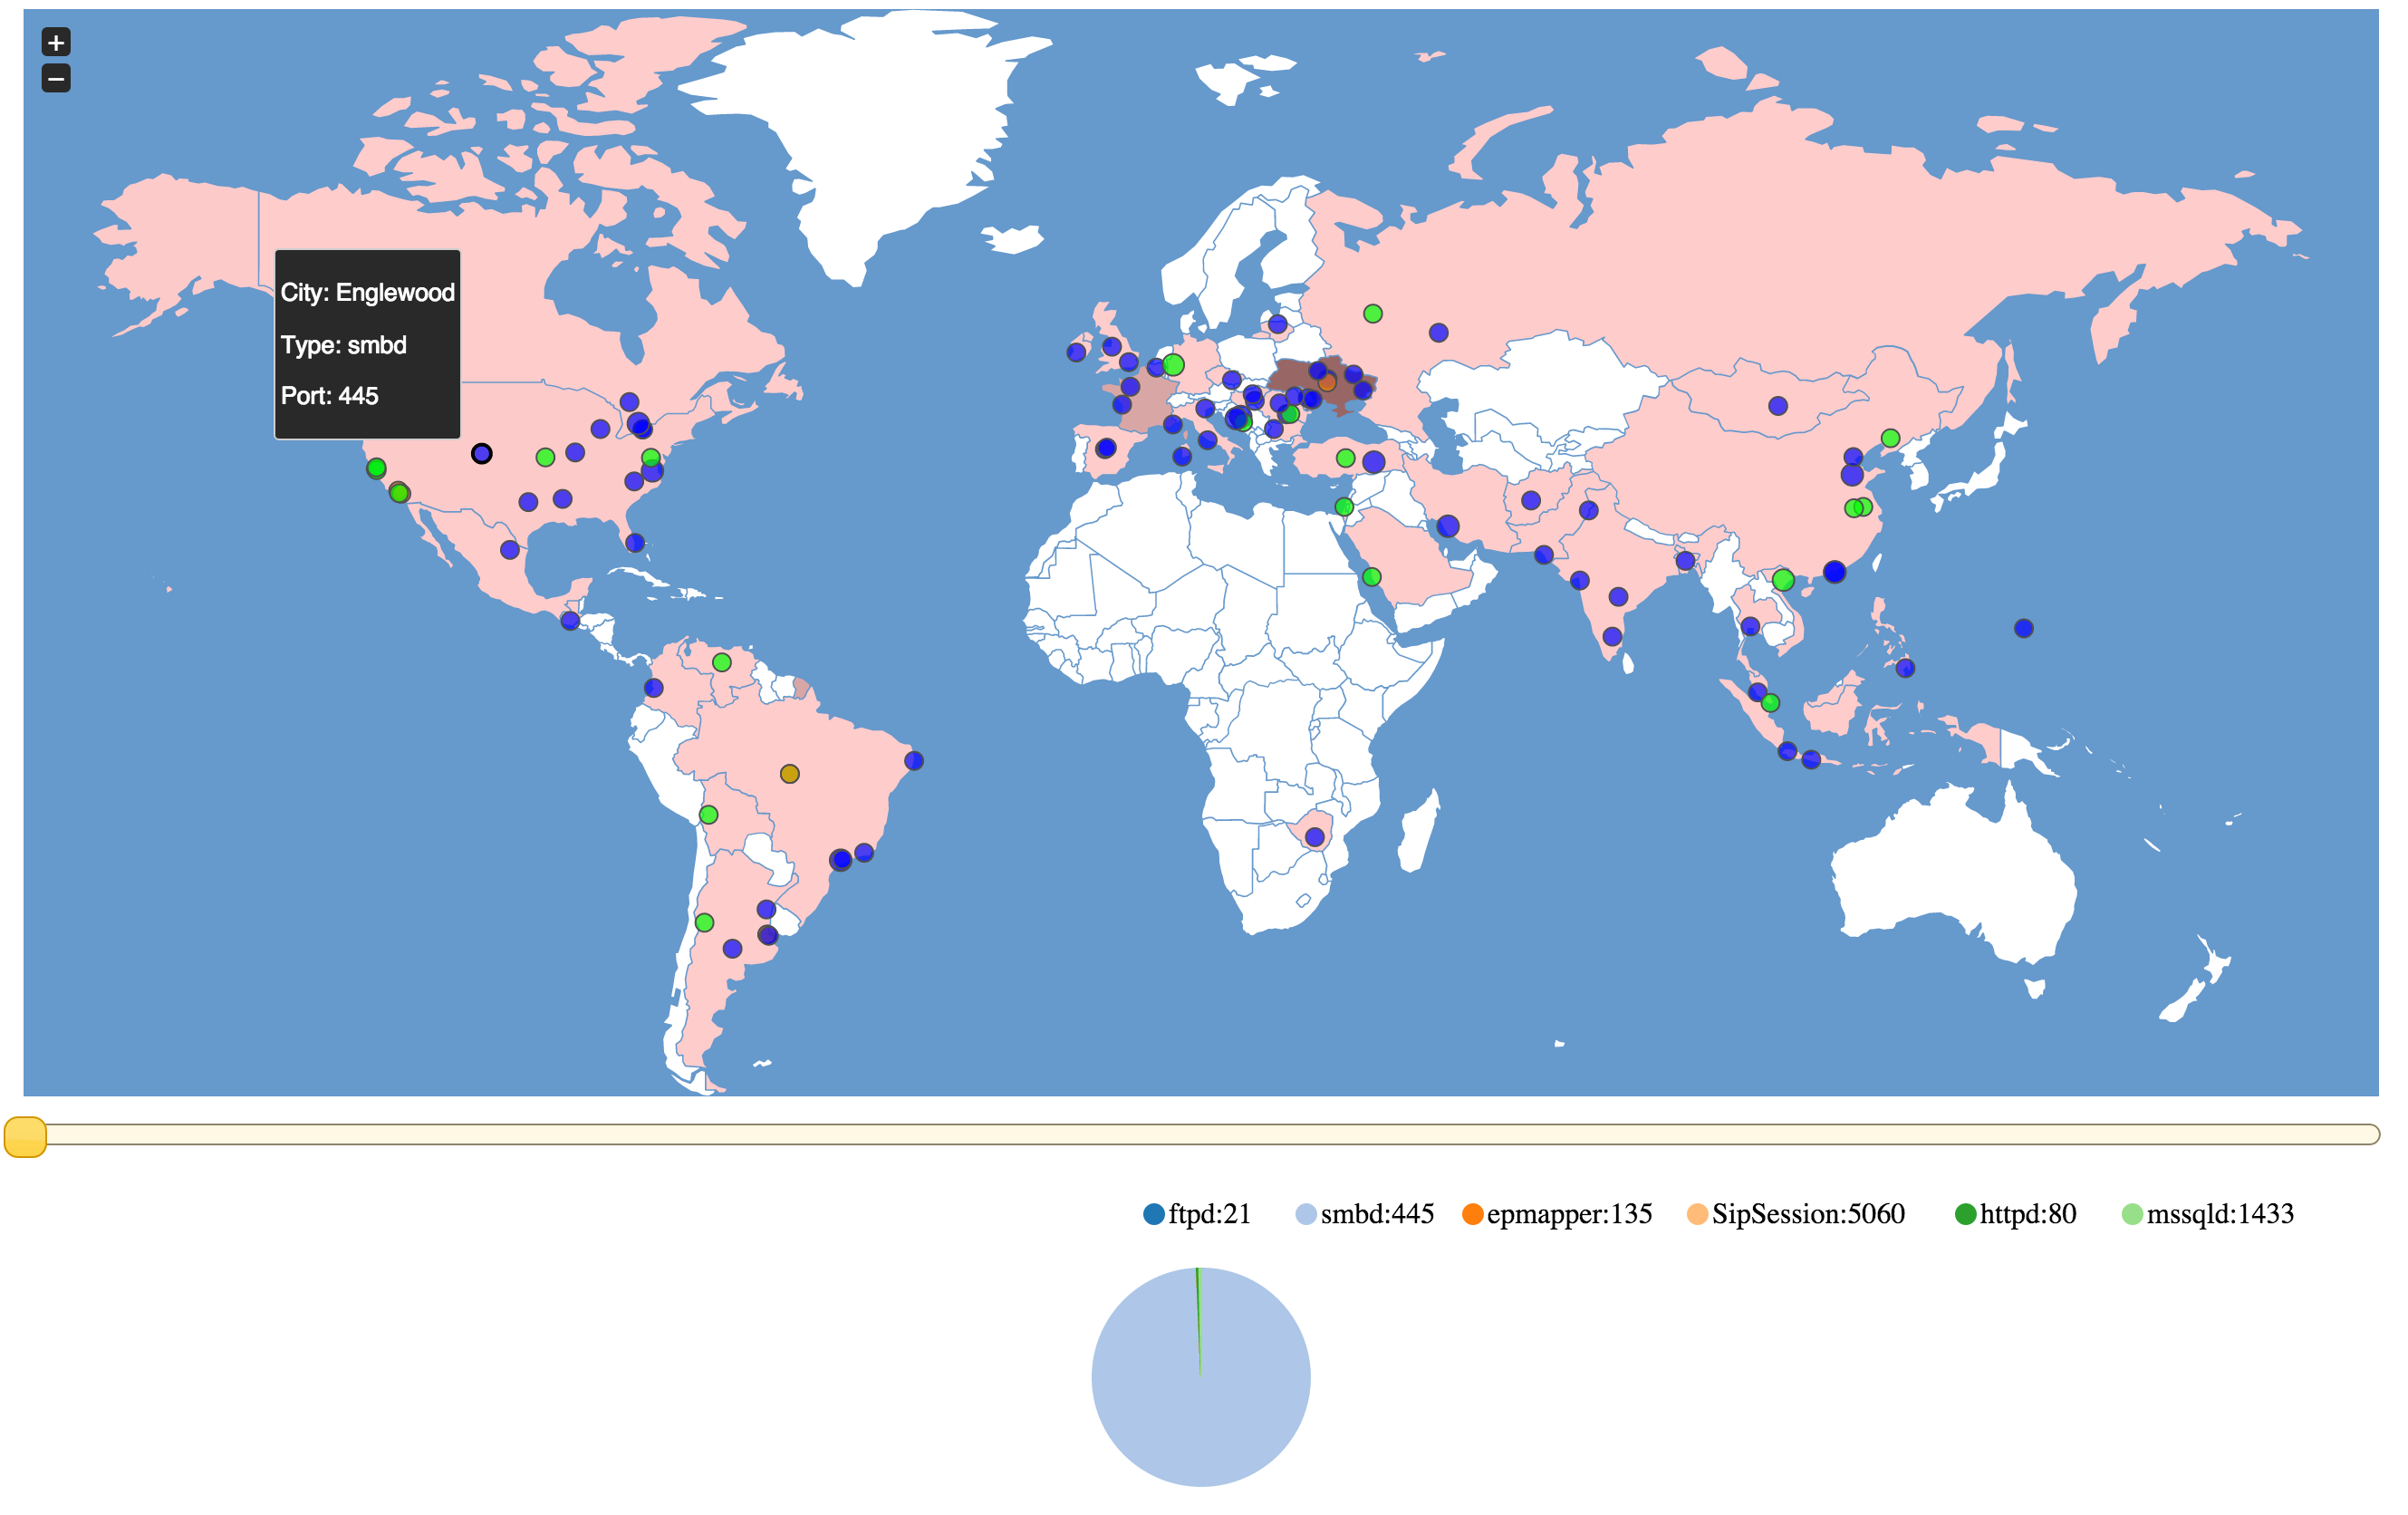
\includegraphics[width=1\textwidth]{figs/mapa.png}
\caption{Mapa mostrado pela interface web retratando os locais de origem dos ataques}
\label{mapa}
\end{figure}


A Figura \ref{mapa} representa um mapa em um dado instante de tempo com dados de potenciais ataques apresentados de acordo com a localização geográfica do endereço IP obtido, bem como outras informações (vide quadro escuro na América do Norte), tais como, a cidade estimada por meio das coordenadas obtidas do IP, o tipo do ataque (serviço alvo) e a porta de rede vulnerável que recebeu o ataque. Logo abaixo do mapa, pode-se notar uma barra de rolagem, a qual movimenta-se de forma automática para mostrar as tendências de ataque ao longo do dia e, mais abaixo, um gráfico que representa os protocolos monitorados e a frequência das conexões recebidas por estes protocolos no instante de tempo em questão.


\chapter{Considerações finais}
Conforme apresentado na seção anterior, foram obtidos resultados concretos no projeto durante o período da bolsa. Entretanto, existem atividades importantes a serem feitas para os futuros trimestres, como previsto no plano de trabalho, as quais irão permitir a obtenção de informações de mais qualidade do ponto de vista de segurança. As principais propostas dessas atividades consistem do desenvolvimento de procedimentos para o tratamento dos dados obtidos, agregação de outros tipos de dados (provenientes de outros sensores) e a correlação de dados de diferentes endereços de origem e fontes visando a descoberta de ataques em associação.

Além disso, há espaço para melhorias no que se refere a usabilidade da ferramenta, entre as quais incluem- se: uma melhor escolha de cores para a representação dos dados no mapa, melhor disposição do gráfico de protocolos, apresentação de mais informações sobre os potenciais ataques e uma interface mais avançada para a manipulação da dimensão temporal dos dados, permitindo ao analista definir intervalos de tempo para apresentar os dados com o objetivo de identificar padrões com maior facilidade.

Por último, pretende-se buscar uma melhoria na performance do sistema em relação ao tempo de resposta entre a busca dos dados no banco de dados e a renderização dos pontos no mapa. Isto é possível por meio do uso de cache e outras técnicas de otimização disponíveis na plataforma Django, mas tais funcionalidades estavam além do escopo do protótipo desenvolvido até o momento.


\chapter{Conhecimentos adquiridos}
\section{Aplicabilidade}
Os conhecimentos adquiridos durante esse projeto possuem uma ampla área de aplicação, sendo esta qualquer área que necessite uma forma visual de interpretar dados. Além disso, a experiência que obtive com a criação de serviços Web e utilização/programação em plataformas e arquiteturas diferentes não possui nenhuma restrição quanto a área de aplicação, podendo ser útil tanto em pesquisas futuras quanto em trabalhos de desenvolvimento.

\section{Incorporação de novas técnicas}
Neste projeto adquiri intimidade com o estilo de programação de APIs no padrão REST, que permite o desenvolvimento de aplicativos Web fracamente acoplados, possibilitando assim a criação de serviços Web escaláveis e capazes de se adaptar a mudança de requisitos de forma flexível. Além disso, familiarizei-me com a plataforma Django, que tem sido muito utilizada em diversos meios, do acadêmico ao industrial, para criação de sistemas Web com diversas características integradas e possibilidade de criação de módulos em Python.

\section{Geração de produtos e processos}
Ao longo do projeto desenvolvi um cliente em JavaScript que permite a visualização de dados não específicos em um mapa de forma genérica, podendo assim ser reutilizado para futuros projetos envolvendo representação de dados nos quais sua posição geográfica possui importância.

Adquiri conhecimento para sobre o processo de geração de imagens em Virtualbox, sendo útil para encapsular sistemas em um ambiente virtual controlado, tornando-o assim portável. Este processo de criação de imagens executáveis (appliances) serve para a preparação de demonstrações de qualquer tipo, tornando- as mais confiáveis ao custo de perda de performance, porém permitindo a disponibilização e utilização de maneira facilitada.

\section{Contribuição da participação no projeto para sua formação}
Participar no projeto contribuiu para o meu conhecimento de ferramentas para rápida prototipagem de aplicações e implantação de serviços Web. Tais conhecimentos não são restritos a área de pesquisa, mas sim também para o mercado de trabalho, onde no modelo atual de startups, o tempo para a execução de um projeto é capaz de determinar o futuro da empresa. Aprendi também a estruturar relatórios técnicos de maneira adequada de forma a expor ideias e mostrar resultados.


\bibliographystyle{plain}
\bibliography{mybib}
\ldots

